\documentclass[11pt]{article}
\usepackage[margin=1in]{geometry}
\usepackage{amssymb}
\usepackage{amsfonts}
\usepackage{amsmath}
\usepackage{graphicx}

\begin{document}

\title{Feasibility of Machine Learning}
\author{Kelvin $\cdot$ Liang \, ziyoustep@gmail.com}
\date{June, 12, 2018}
\maketitle

\section{Introduction}
In this note, we are going to address the feasibility of learning from probability side of perspective. We will show how limited known data set $\mathbb{D}$ reveal enough information about the unknown target function $f$. Before the discussion of the feasibility of learning we need to introduce the very most important \textbf{Hoeffding Inequality} first.

\section{Hoeffding Inequality}

For any sample size $N$\\
\begin{eqnarray}
P\left(|\overline{X} - E(\overline{X})| > \epsilon\right) \leq 2e^{-2\epsilon^2 N} \qquad, for \, any \, \epsilon > 0
\end{eqnarray}

Here is what each notation means\\ 
\begin{itemize}
\item $N:$ Sample size \\
\item $P():$ Probability of an event\\
\item $\displaystyle{\overline{X}:\frac{X_1+ \cdots +X_N}{N}}$ \qquad \qquad$X_i$ is i.i.d random variable\\
\item $E(\overline{X}):$ Expectation of $\overline{X}$\\
\item $\epsilon:$ Any positive value that we chose
\end{itemize}
The inequality above says that, as long as $N$ gets large enough $\overline{X}$ will approximate to ${E(\overline{X})}$. That is we can infer ${E(\overline{X})}$ by $\overline{X}$. We are going to use this inequality to explain why machine learning is feasible.

\section{Applying Hoeffding Inequality to Machine Learning Feasibility Problem}
We first define In-sample error and out-of-sample error which are corresponding to $\overline{X}$ and $E(\overline{X})$ respectively.

\textbf{In-sample error}\\
\begin{eqnarray}
\displaystyle{E_{in}(h) = \frac{1}{N} \sum _{i=1}^{N} \left[ isTrue\left( h(x_i) \neq f(x_i) \right) \right]}
\end{eqnarray}

\textbf{Out-of-sample error}\\
\begin{eqnarray}
\displaystyle{E_{out}(h) = P[h(x) \neq f(x)]}
\end{eqnarray}

We plug them into Hoeffding Inequality and get
\begin{eqnarray}
P\left(|E_{in}(h) - E_{out}(h)| > \epsilon\right) \leq 2e^{-2\epsilon^2 N} \qquad, for \, any \, \epsilon > 0
\end{eqnarray}
\\
As of the original Hoeffding Inequality, we can say that $E_{in}(h)\to E_{out}(h)$ as $N$ increase. But, before we can state this conclusion, we must ensure that the sampling data(training data) $\mathbb{D}$ fulfill some requirements. For the reason that the random variables$(X_1, X2, \cdots , X_N)$ that we used to calculate $\overline{X}$ are all identical independent random variables(i.i.d). So, the training data of our machine learning model need to follow this requirement as well. To generate a training data set with i.i.d random variables, we need an input distribution $\textbf{Distri(X)}$ which can produce i.i.d $(X_1, X2, \cdots , X_N)$ for us. The function of this input distribution is illustrated in the structure graph below.

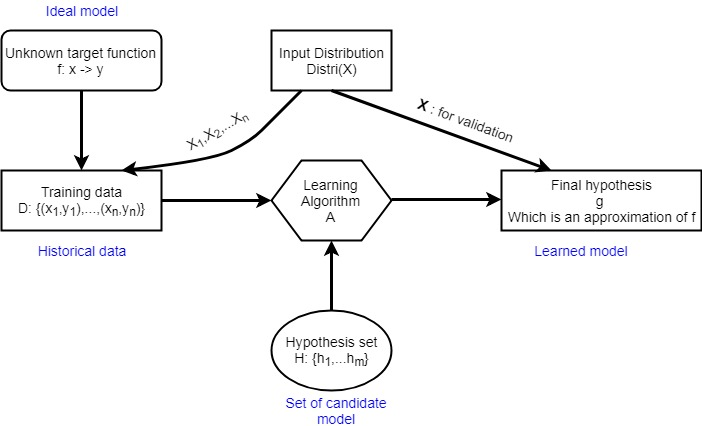
\includegraphics[scale=0.62]{ProbabilityLearningModel.jpg}\\

Now we can say that $E_{in}(h)\approx E_{out}(h)$ as $N$ gets large enough. But it doesn't implies that $h\approx f$. What we need to do now is to find out a $g$ from the hypothesis set $\mathbb{H}$, so that $E_{in}(g)$ is as small as possible. Then, we have $E_{in}(g)\approx 0 \to E_{out}(g)\approx 0$. By the definition of $E_{out}(g)$, we know that $g \approx f$ if $E_{out}(g) \approx 0$.

Here, the feasibility of machine learning is thus split into two questions.
\begin{enumerate}
\item How to make $E_{in}(g)$ close enough to $E_{out}(g)$.\\
\item How to make $E_{in}(g)$ as small as possible.
\end{enumerate}

But, There are still some problems that we need to clarify about $g$. The probability upper bound of $g$ is larger than $h$ for the reason that we manually chose it from the hypothesis set. This manual selection make $g$ easier to become a poor estimator. We will prove this in the following section.

\section{Problems Caused by the Size of Hypothesis Set}
We start by introducing to basic probability rules.

$$\textbf{Rule 1.}\qquad If A \Rightarrow B, then P(A) \leq P(B)$$
$$\textbf{Rule 2.}\qquad P(A_1|A_2|\cdots |A_m) \leq P(A_1) + P(A_2) + \cdots + P(A_m)$$
Now, we are going to illustrate the problem caused by manual selection of $g$. Suppose there are $m$ hypothesis in $\mathbb{H}$. Then we have

\begin{eqnarray*}
&P&\left(|E_{in}(h_1) - E_{out}(h_1)| > \epsilon\right) \leq 2e^{-2\epsilon^2 N} \qquad, for \, any \, \epsilon > 0\\
&P&\left(|E_{in}(h_2) - E_{out}(h_2)| > \epsilon\right) \leq 2e^{-2\epsilon^2 N} \qquad, for \, any \, \epsilon > 0\\
&\cdots& \\
&P&\left(|E_{in}(h_m) - E_{out}(h_m)| > \epsilon\right) \leq 2e^{-2\epsilon^2 N} \qquad, for \, any \, \epsilon > 0
\end{eqnarray*}

Because $g$ is one of $h_i$ we have

\begin{eqnarray*}
|E_{in}(g) - E_{out}(g)| > \epsilon \Rightarrow &"& |E_{in}(h_1) - E_{out}(h_1)| > \epsilon\\
&or& |E_{in}(h_2) - E_{out}(h_2)| > \epsilon\\
&\cdots& \\
&or& |E_{in}(h_m) - E_{out}(h_m)| > \epsilon "
\end{eqnarray*}

By applying Rule 1 and Rule 2, we easily get

\begin{eqnarray}
P[|E_{in}(g) - E_{out}(g)| > \epsilon] &\leq& \sum _{i=1}^{m}P[|E_{in}(h_i) - E_{out}(h_i)| > \epsilon]\\
&\leq& 2me^{-2\epsilon^2 N}
\end{eqnarray}

As is clearly shown on equation (6), The upper bound of $g$ increase as the size hypothesis set $\mathbb{H}$ increase. Here comes the dilemma of machine learning. If we want $E_{in}(g)$ to be smaller, we need to increase the size of $\mathbb{H}$. But this will make $E_{in}(g)$ deviate from $E_{out}(g)$. If we want $E_{in}(g)$ to be closer to $E_{out}(g)$, we need to decrease the size of $\mathbb{H}$. But this will make $E_{in}(g)$ gets larger and lead to the deviation of $g$ from $f$. We will discuss how to balance the two sides of a coin in later notes. 

\section{References}
Almost all of the materials of this note are from Professor Hsuan-Tien Lin , NTU. If you wan to know more information about Machine Learning Foundation, please refer to Professor Lin's homesite.

\end{document}